\exercise{Timer}
Si realizzi la classe \cod{Timer} che svolga le funzioni di cronometro. Tale oggetto deve poter gestire i messaggi START, STOP, RESET e GETTIME comportandosi come specificato dall'interfaccia seguente.

\begin{methodslist}

\method{Start}{\emptyset}{\emptyset}{
Avvia il conteggio del tempo.
}

\method{Stop}{\emptyset}{\emptyset}{
Arresta il conteggio del tempo.
}

\method{Reset}{\emptyset}{\emptyset}{
Arresta ed azzera il timer.
}

\method{GetTime}{\emptyset}{Time}{
Restituisce il conteggio corrente del tempo.
}

\end{methodslist}

Nella figura � riportato un esempio grafico del funzionamento dell'oggetto.

\begin{figure}
  \center
	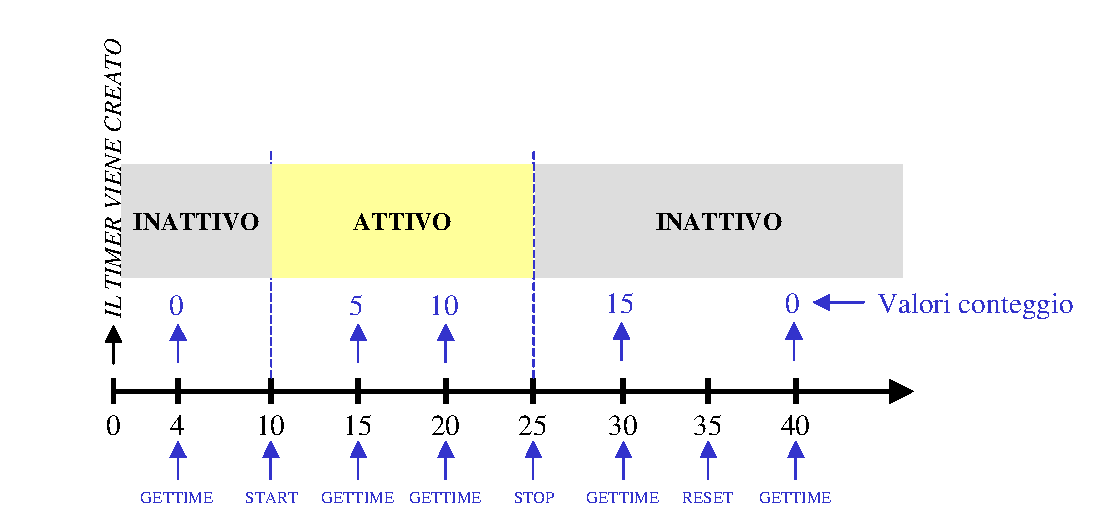
\includegraphics[width=.9\textwidth]{Esercizi/Timer/Timer.eps}
	\caption{Un esempio d'uso del timer nel tempo}
	\label{fig:Timer}	
\end{figure}

\subsubsection*{Suggerimenti}
\begin{itemize}
\item
La seguente riga di codice:
\begin{codequote}
  time t = time(0);
\end{codequote}
istanzia una variabile \cod{t} di tipo \cod{time} e la pone uguale al tempo di sistema, restituito dalla funzione \cod{time()}, sotto la forma di un intero che rappresenta il numero di secondi trascorsi dalla mezzanotte del 1 gennaio 1970. La funzione \cod{time()} � presente nella libreria C \cod{time.h}.
\item
Il funzionamento del timer nei casi non espressamente previsti dalle specifiche sia arbitrario.
\end{itemize}